\documentclass{article}
\usepackage{graphicx}
\usepackage{float}

\title{doc}
\author{Valentina piscopo}
\date{August 2025}

\begin{document}

\maketitle

\tableofcontents
\newpage

\section{Introduzione}

Quando ci affidiamo ai metodi di spiegazione per i modelli di \emph{machine
      learning}, nasce una domanda fondamentale: \textit{quanto sono simili tra loro
      le spiegazioni prodotte da diversi algoritmi o modelli, e come è possibile
      misurare questa similarità?}

Nel contesto del \emph{Rashomon effect}, in cui si osserva la coesistenza di
molteplici modelli con prestazioni equivalenti ma parametri differenti, questa
domanda diventa ancora più centrale: se più modelli ottengono gli stessi
risultati, ci aspettiamo che le loro decisioni vengano spiegate nello stesso
modo?

Per affrontare questa questione si può procedere nel seguente modo:
\begin{enumerate}
      \item Costruire un setup sperimentale in cui diversi modelli, ugualmente accurati,
            vengano analizzati con uno o più metodi di spiegazione.
      \item Applicare diverse metriche di similarità alle spiegazioni ottenute, ad esempio
            lo \emph{Structural Similarity Index} (SSIM), la correlazione di Pearson, la
            similarità coseno, ecc.
      \item Confrontare i risultati delle metriche per capire se, e quanto, variano le
            spiegazioni a seconda del modello e del metodo utilizzato.
\end{enumerate}

Tuttavia, emergono alcune criticità:
\begin{itemize}
      \item Spiegazioni diverse producono valori di similarità differenti anche per lo
            stesso input. Due metodi di spiegazione potrebbero identificare feature diverse
            come rilevanti.
      \item Due metriche diverse potrebbero restituire giudizi contrastanti sul grado di
            similarità.
      \item Non sempre è chiaro quale spiegazione sia migliore: una spiegazione più simile
            a un’altra non è automaticamente più fedele o più utile; spesso manca un
            \emph{ground truth} oggettivo della spiegazione ideale.
\end{itemize}

La qualità di una spiegazione va quindi oltre la sola similarità: per capire se
una spiegazione è effettivamente efficace, occorre valutarne anche la
\emph{fedeltà} al funzionamento reale del modello. Un approccio diffuso a
questo scopo è l’analisi mediante curve \emph{MoRF} (\emph{Most Relevant
      First}): si mascherano progressivamente le feature considerate importanti dalla
spiegazione e si osserva quanto rapidamente decresce la confidenza del modello.

Ad esempio, immaginiamo una rete neurale che riconosce un gatto in una foto: se
la spiegazione individua le orecchie come la feature più rilevante e,
rimuovendole, la probabilità che il modello predica “gatto” cala drasticamente,
allora la spiegazione si dimostra fedele. Se invece la predizione cambia di
poco, la spiegazione perde significato.

In letteratura non esiste una metrica unica e definitiva per confrontare o
valutare le spiegazioni; piuttosto, si adottano più prospettive complementari,
mettendo a confronto i risultati tra metodi e modelli diversi, e integrando
valutazioni di similarità con misure di fedeltà come MoRF.

\section{Introduzione all’implementazione sperimentale}

L’esperimento è stato strutturato come una pipeline in più fasi, ciascuna con
un obiettivo specifico:

\begin{enumerate}
      \item \textbf{Costruzione di un Rashomon set}: una raccolta di modelli differenti, ma tutti con prestazioni simili sullo stesso compito di classificazione.
      \item \textbf{Applicazione di metodi di spiegazione}: generazione di spiegazioni locali per ciascun modello, su un insieme di dati di test, utilizzando diversi algoritmi XAI.
      \item \textbf{Valutazione della similarità delle spiegazioni}: confronto quantitativo tra le spiegazioni prodotte da modelli e metodi differenti, tramite varie metriche di similarità.
      \item \textbf{Valutazione della fedeltà delle spiegazioni}: misurazione di quanto le feature individuate dalle spiegazioni siano realmente determinanti per le predizioni dei modelli, mediante tecniche come le curve \emph{MoRF}.
\end{enumerate}

\subsection{Tecnologie}
Per implementare il workflow sperimentale descritto, è stato utilizzato un
ecosistema di strumenti largamente adottati in ambito \emph{explainable AI}, in
grado di garantire affidabilità, riproducibilità e scalabilità:

\begin{itemize}
      \item \textbf{Python 3.x}: linguaggio di riferimento per la ricerca in XAI, scelto per la sua flessibilità e l’ampia disponibilità di librerie specializzate.
      \item \textbf{PyTorch}: libreria \emph{open-source} per il \emph{machine learning} e \emph{deep learning}, dotata di supporto nativo per l’autograd e adatta alla prototipazione rapida di modelli. Utilizzata per la definizione, l’addestramento e la validazione delle reti neurali, nonché per il calcolo dei gradienti richiesto dai metodi \emph{Saliency} e \emph{Integrated Gradients}.
      \item \textbf{Torchvision}: libreria complementare a PyTorch che offre dataset predefiniti (come MNIST), trasformazioni standard per immagini e modelli già pronti. Utilizzata per il download, la gestione e il preprocessing del dataset MNIST.
      \item \textbf{Captum}: libreria open source specifica per l’interpretabilità di modelli PyTorch. Fornisce implementazioni ottimizzate di numerosi metodi XAI, con API coerenti e facilmente integrabili. Utilizzata per generare le spiegazioni su tutti i modelli del Rashomon set, includendo metodi \emph{gradient-based} e \emph{model-agnostic}.
      \item \textbf{NumPy}: libreria fondamentale per il calcolo scientifico e la manipolazione efficiente di array numerici, usata per l’elaborazione dei dati, la normalizzazione delle spiegazioni e il calcolo di metriche.
      \item \textbf{Scikit-learn}: utilizzata per il calcolo di metriche (correlazioni, MAE) e per funzioni di utilità scientifica.
      \item \textbf{SciPy}: impiegata per calcolare correlazioni avanzate come Spearman e Pearson.
      \item \textbf{Scikit-image}: usata per il calcolo della metrica \emph{SSIM} (\emph{Structural Similarity Index}).
      \item \textbf{Matplotlib}: libreria di riferimento per la visualizzazione scientifica, utilizzata per produrre grafici e visualizzazioni qualitative delle spiegazioni.
      \item \textbf{Tqdm}: per fornire barre di avanzamento e monitorare l’esecuzione di processi lunghi.
      \item \textbf{Glob, os}: per la gestione di file, directory e per il caricamento/salvataggio dei modelli, a supporto della riproducibilità.
\end{itemize}

\subsection{Riproducibilità e ambiente di sviluppo}
Per garantire la riproducibilità degli esperimenti e la gestione efficiente
delle dipendenze, sono state adottate le seguenti buone pratiche:
\begin{itemize}
      \item \textbf{Gestione dell’ambiente con \emph{conda}}: tutte le dipendenze (librerie e relative versioni) sono state installate in un ambiente dedicato, così da poter replicare esattamente il contesto di esecuzione.
      \item \textbf{Controllo della casualità}: i \emph{random seed} sono stati fissati per NumPy, PyTorch e il generatore casuale di Python, così da rendere i risultati ripetibili anche in presenza di componenti stocastiche come l’inizializzazione dei pesi o lo \emph{shuffle} dei dati.
      \item \textbf{Salvataggio e caricamento dei modelli}: i modelli selezionati per il Rashomon set sono stati salvati su disco durante la fase di addestramento, evitando la ripetizione di processi costosi e permettendo il loro riutilizzo in fasi successive.
\end{itemize}

\subsection{Scelte implementative}

Tutti gli esperimenti sono stati condotti utilizzando \textbf{CPU} anziché GPU,
condizione che ha influenzato alcune scelte implementative per mantenere tempi
di esecuzione ragionevoli.

\begin{itemize}
      \item \textbf{LIME:} è stato adottato un approccio \textit{patch-based} su immagini MNIST ($28\times28$ pixel), con suddivisione in blocchi $4\times4$ (\texttt{feature\_mask}) per un totale di 49 feature. Questa scelta riduce drasticamente il rumore rispetto a una perturbazione a livello di singolo pixel (784 feature), aumentando la stabilità delle spiegazioni e riducendo il tempo di calcolo. Il numero di campioni per LIME è stato fissato a $n\_samples = 1000$, per aumentare la stabilità delle spiegazioni rispetto a un numero minore di campioni. Questa scelta, pur aumentando i tempi di calcolo su CPU, è stata resa sostenibile grazie all’uso di \texttt{perturbations\_per\_eval=50}, che consente di elaborare batch di perturbazioni in parallelo riducendo l’overhead.

      \item \textbf{Integrated Gradients (IG):} è stato utilizzato il numero di passi predefinito di Captum (\texttt{n\_steps} di default), con baseline impostata a un’immagine di zeri. Questo riduce i costi di calcolo evitando sampling multipli.

      \item \textbf{Saliency:} calcolata con il metodo standard di Captum senza smoothing addizionale, per mantenere la velocità di esecuzione e non introdurre bias dovuto a parametri aggiuntivi.

      \item \textbf{MoRF/AOPC:} la mascheratura progressiva utilizza 10 step, sostituendo le feature con la \textit{media dell’immagine} come baseline. Questa scelta minimizza l’impatto visivo di feature rimosse mantenendo tempi computazionali bassi.

      \item \textbf{Selezione del Rashomon set:} i modelli vengono scelti in base alla \textit{validation accuracy}, con soglia di Rashomon fissata all’1\% rispetto al miglior modello. Per ogni modello salvato, si memorizza lo stato in formato \texttt{.pt} di PyTorch.
\end{itemize}

In tutti i casi, le attribuzioni sono calcolate rispetto alla \textbf{classe
      vera} (\textit{true label}) e non rispetto alla classe predetta. Questa scelta
è stata effettuata per garantire coerenza con il \textit{ground truth} ed
evitare che eventuali errori di predizione introducano variazioni spurie nelle
spiegazioni. Tuttavia, ciò rappresenta una possibile minaccia alla validità
esterna, poiché in scenari reali la classe vera non è nota all’utente finale.

\subsection{Hyperparametri e setup sperimentale}

Nella Tabella~\ref{tab:hyperparams} sono riportati tutti i parametri e le
impostazioni utilizzate negli esperimenti, in modo da permettere la
riproducibilità dei risultati.

\begin{table}[H]
      \centering
      \renewcommand{\arraystretch}{1.2}
      \begin{tabular}{ll}
            \hline
            \textbf{Parametro}              & \textbf{Valore}                                             \\
            \hline
            Numero di modelli addestrati    & 10                                                          \\
            Epoche massime                  & 50                                                          \\
            Patience (early stopping)       & 5 epoche                                                    \\
            Soglia Rashomon                 & $1\%$ di differenza rispetto al miglior modello (val. acc.) \\
            Batch size                      & 128                                                         \\
            Baseline IG                     & immagine di zeri                                            \\
            Baseline MoRF                   & media dell’immagine                                         \\
            $n\_samples$ LIME               & 1000                                                        \\
            Feature mask LIME               & blocchi 4×4 (49 feature totali)                             \\
            $n\_steps$ IG                   & valore predefinito Captum                                   \\
            Step MoRF                       & 10                                                          \\
            Classe di riferimento           & Classe vera (\textit{true label})                           \\
            Ottimizzatore                   & Adam                                                        \\
            Tasso di apprendimento iniziale & 0.001                                                       \\
            Dataset                         & MNIST (grayscale, 28×28)                                    \\
            \hline
      \end{tabular}
      \caption{Hyperparametri e setup utilizzati negli esperimenti.}
      \label{tab:hyperparams}
\end{table}

\section{Il Rashomon set}

Il \emph{Rashomon set} è una collezione di modelli diversi che ottengono
prestazioni simili su un determinato compito. Prende il nome dall’effetto
Rashomon, che descrive la possibilità che più spiegazioni, tutte coerenti con i
dati osservati, possano emergere per lo stesso fenomeno. In ambito
\emph{machine learning}, questo implica che, anche a parità di accuratezza,
modelli con parametri differenti possono fornire spiegazioni distinte per le
proprie decisioni.

\subsection{Costruzione}
Il Rashomon set è stato costruito allenando più reti neurali della stessa
architettura (una CNN semplice) sul dataset MNIST. Ogni rete parte da una
diversa inizializzazione casuale dei pesi (\emph{random seed} differente) ed è
addestrata sugli stessi dati con un protocollo identico, che include la
suddivisione in training, validation e test set.

Durante l’addestramento è stata applicata la tecnica di \emph{early stopping}:
per ogni modello, l’allenamento viene interrotto se le prestazioni sul
validation set non migliorano per un numero prestabilito di epoche consecutive.
In questo modo si seleziona automaticamente la versione del modello che ha
ottenuto la miglior accuratezza sul validation, riducendo il rischio di
overfitting.

\subsection{Selezione}
Al termine dell’addestramento, sono stati selezionati tutti i modelli che
ottenevano un’accuratezza sul validation entro una certa soglia rispetto al
modello con la miglior performance. In questo esperimento la soglia è pari
all’1\%:

\[
      \mathrm{Accuracy}_{\mathrm{val}}(m) \geq \mathrm{Accuracy}_{\mathrm{val}}(m_{\mathrm{best}}) - \epsilon
\]
dove:
\begin{itemize}
      \item $\mathrm{Accuracy}_{\mathrm{val}}(m_{\mathrm{best}})$ è la miglior accuratezza sul validation ottenuta tra tutti i modelli addestrati;
      \item $\epsilon$ è la tolleranza fissata (0.01 in questo caso).
\end{itemize}

Questo criterio garantisce che i modelli del Rashomon set siano equivalenti dal
punto di vista delle prestazioni, pur potendo avere rappresentazioni interne e
logiche decisionali differenti.

\subsection{Obiettivi}
La costruzione del Rashomon set serve a due scopi principali:
\begin{enumerate}
      \item \textbf{Studiare la variabilità delle spiegazioni}: se modelli ugualmente accurati forniscono spiegazioni simili, allora queste possono essere considerate robuste; se divergono, si manifesta l’effetto Rashomon anche nell’interpretabilità.
      \item \textbf{Testare i metodi di spiegazione}: usando un insieme di modelli equivalenti, è possibile valutare la coerenza e la fedeltà delle spiegazioni prodotte da diversi algoritmi XAI.
\end{enumerate}

\subsection{Approfondimento: equivalenza tra modelli}
Nel contesto di questo lavoro, due modelli sono considerati equivalenti se
soddisfano la condizione di soglia sull’accuratezza definita sopra. Questa
scelta è in linea con la letteratura, in quanto:
\begin{itemize}
      \item Rispetta la definizione originaria di Rashomon set come insieme di modelli con
            prestazioni quasi ottimali.
      \item Permette di esplorare la diversità interna tra modelli che, in termini
            predittivi, sembrano “uguali”.
\end{itemize}

\subsection{Perché utilizzare l’early stopping}
L’\emph{early stopping} è stato adottato per due motivi principali:
\begin{itemize}
      \item \textbf{Evitare l’overfitting}: interrompendo l’addestramento quando le prestazioni di validazione smettono di migliorare, si evita che il modello memorizzi il training set perdendo capacità di generalizzazione.
      \item \textbf{Equità nel confronto}: applicando la stessa regola a tutti i modelli, ciascun membro del Rashomon set viene selezionato nelle condizioni di miglior equilibrio tra bias e varianza.
\end{itemize}

Questo approccio assicura che la variabilità osservata nelle spiegazioni non
sia dovuta a un diverso grado di overfitting, ma a reali differenze nei
percorsi di apprendimento.

\subsection{Riproducibilità dei risultati}
La replicabilità degli esperimenti è stata garantita mediante:
\begin{itemize}
      \item Inizializzazione di ciascun modello con un \emph{seed} diverso, per generare
            percorsi di apprendimento unici.
      \item Fissaggio dei \emph{random seed} di NumPy e PyTorch, così da rendere
            deterministico il processo di addestramento.
\end{itemize}

In questo modo, è possibile distinguere la variabilità dovuta al caso da quella
legata a differenze strutturali nei modelli o nelle spiegazioni.

\section{Metodi di spiegazione adottati}

Una volta selezionato il \emph{Rashomon set} dei modelli, il passo successivo
consiste nell’analizzare come ciascun modello giunge alle proprie decisioni.
Per questo scopo sono stati utilizzati tre metodi di spiegazione, scelti per
rappresentare sia approcci \emph{gradient-based} che \emph{model-agnostic}.

\subsection{Saliency}
Il metodo della \emph{saliency map} è uno dei più semplici e diffusi. Calcola
la derivata della probabilità (o della logit) assegnata dal modello alla classe
target rispetto a ciascun pixel dell’immagine di input. I pixel associati ai
valori assoluti più elevati sono considerati più importanti per la decisione.
Questo metodo è apprezzato per la sua immediatezza, ma è noto per essere
sensibile al rumore e all’inizializzazione dei pesi del modello.

\subsection{Integrated Gradients (IG)}
Gli \emph{Integrated Gradients} migliorano l’approccio delle saliency map,
correggendone alcune limitazioni. Calcolano il contributo di ogni feature
effettuando una media dei gradienti lungo un percorso che va da una
\emph{baseline} (nel nostro caso, immagine nulla) fino all’immagine reale.
Questo consente di ottenere spiegazioni più stabili e coerenti, meno
influenzate da piccole variazioni nei dati o nei parametri del modello.

\subsection{LIME}
Il metodo \emph{LIME} (\emph{Local Interpretable Model-agnostic Explanations})
genera nuove istanze di input perturbate (ad esempio, oscurando casualmente
parti dell’immagine) e osserva come cambia la predizione del modello.
Successivamente, addestra un modello interpretabile locale (ad esempio una
regressione lineare) per stimare quali feature hanno avuto il maggiore impatto
sulla decisione del modello. Nel caso di MNIST, le perturbazioni sono
effettuate a livello di singolo pixel, senza segmentazione in super-pixel.

\subsection{Motivazioni della scelta}
La combinazione di questi tre metodi consente di confrontare:
\begin{itemize}
      \item Approcci \emph{gradient-based} (Saliency, IG) e approcci \emph{model-agnostic}
            (LIME).
      \item Metodi semplici e veloci con tecniche più robuste e computazionalmente costose.
      \item Stabilità delle spiegazioni e capacità di cogliere diversi aspetti
            dell’importanza delle feature.
\end{itemize}

\subsection{Gradient-based vs Model-agnostic}
I metodi di spiegazione \emph{gradient-based} sfruttano direttamente la
struttura interna del modello: calcolano come varia la predizione rispetto a
piccole modifiche delle feature in input, utilizzando le derivate calcolate
tramite \emph{backpropagation}. Questi metodi sono veloci e, per modelli
differenziabili come le reti neurali, forniscono indicazioni precise sulle
feature che guidano la decisione.

I metodi \emph{model-agnostic}, invece, trattano il modello come una “scatola
nera”: non richiedono accesso ai pesi o ai gradienti, ma solo la possibilità di
effettuare predizioni su input modificati. Questo li rende molto flessibili
(applicabili a qualsiasi modello), ma spesso più lenti e meno stabili, poiché
si basano su approssimazioni locali.

\section{Valutare la similarità tra spiegazioni}

Quando osserviamo due spiegazioni, possiamo essere tentati di giudicare ``a
occhio'' se siano simili o meno. Ma le apparenze ingannano: differenze visive
possono non riflettere reali differenze nei pattern di importanza, e viceversa.
Nel contesto di un \emph{Rashomon set}, questa domanda diventa cruciale:
modelli diversi, ma ugualmente accurati, arrivano alle stesse conclusioni per
motivi simili, o per motivi profondamente diversi? Misurare la similarità tra
spiegazioni è un passo fondamentale per capire la robustezza e la stabilità
delle interpretazioni fornite dai metodi di \emph{eXplainable AI} (XAI).

\subsection{Metriche adottate}
Per trasformare un concetto qualitativo come ``somiglianza visiva'' in numeri,
è necessario scegliere metriche che catturino aspetti diversi della relazione
tra due mappe di importanza:

\begin{itemize}
      \item \textbf{Structural Similarity Index (SSIM)} — valuta quanto due mappe siano simili in termini di struttura, considerando luminanza, contrasto e distribuzione spaziale. Un SSIM vicino a 1 indica che le due spiegazioni hanno pattern strutturali quasi identici.
      \item \textbf{Pearson correlation} — misura la correlazione lineare tra i valori di importanza, utile per capire se i valori crescono e decrescono insieme, indipendentemente dall’ordine dei pixel.
      \item \textbf{Spearman correlation} — analizza la correlazione tra i ranghi, quindi l’ordine relativo delle feature più importanti, anche se le scale numeriche sono diverse.
      \item \textbf{Cosine similarity} — confronta la direzione dei vettori di importanza, ignorando la loro lunghezza: due spiegazioni che mettono in evidenza le stesse zone avranno un valore vicino a 1, anche se una è “più intensa” dell’altra.
      \item \textbf{Mean Absolute Error (MAE)} — fornisce una misura diretta della differenza media assoluta nei valori di importanza; più è basso, più le mappe sono simili in valore assoluto.
\end{itemize}

La scelta di queste metriche consente di catturare diverse sfaccettature della
similarità: dalla struttura globale all’ordine delle feature, fino alla
corrispondenza numerica esatta.

\subsection{Procedura di confronto}
Il confronto è stato condotto calcolando le metriche per ogni immagine del test
set e per ogni coppia di spiegazioni, in due scenari distinti:

\begin{enumerate}
      \item \textbf{Intra-modello} — confronto tra metodi diversi applicati allo stesso modello. Qui si misura la coerenza tra approcci di spiegazione differenti: se producono mappe simili, il modello è interpretato nello stesso modo indipendentemente dal metodo.
      \item \textbf{Inter-modello} — confronto dello stesso metodo applicato a modelli diversi all’interno del \emph{Rashomon set}. In questo caso si valuta la stabilità del metodo rispetto a variazioni nella struttura interna del modello.
\end{enumerate}

Le attribuzioni sono calcolate sempre rispetto alla \textbf{classe vera}
(\textit{true label}). Questa scelta è stata fatta per garantire coerenza con
il \emph{ground truth} ed evitare che errori di classificazione alterino il
confronto. Tuttavia, rappresenta una potenziale minaccia alla validità esterna:
in scenari reali, la classe vera potrebbe non essere disponibile, e il
comportamento rispetto alla classe predetta potrebbe differire.

\subsection{Risultati quantitativi}
Le tabelle seguenti riassumono i valori medi delle metriche nei due scenari.

\begin{table}[h!]
      \centering
      \renewcommand{\arraystretch}{1.1}
      \begin{tabular}{lccccc c}
            \hline
            \textbf{Coppia} & \textbf{SSIM} & \textbf{Pearson} & \textbf{Spearman} & \textbf{Cosine} & \textbf{MAE} & \textbf{n} \\
            \hline
            Saliency–IG     & 0.263         & 0.529            & 0.194             & 0.651           & 0.211        & 100        \\
            Saliency–LIME   & 0.213         & 0.477            & 0.424             & 0.658           & 0.151        & 100        \\
            IG–LIME         & 0.265         & 0.430            & 0.224             & 0.725           & 0.185        & 100        \\
            \hline
      \end{tabular}
      \caption{Similarità \emph{intra-modello}: confronto tra metodi diversi sullo stesso modello (medie; dallo script non sono disponibili le deviazioni standard).}
      \label{tab:sim_intra}
\end{table}

\begin{table}[h!]
      \centering
      \renewcommand{\arraystretch}{1.1}
      \begin{tabular}{lccccc c}
            \hline
            \textbf{Metodo} & \textbf{SSIM} & \textbf{Pearson} & \textbf{Spearman} & \textbf{Cosine} & \textbf{MAE} & \textbf{n} \\
            \hline
            Saliency        & 0.439         & 0.612            & 0.688             & 0.727           & 0.069        & 450        \\
            IG              & 0.711         & 0.723            & 0.516             & 0.970           & 0.083        & 450        \\
            LIME            & 0.732         & 0.906            & 0.647             & 0.936           & 0.079        & 450        \\
            \hline
      \end{tabular}
      \caption{Similarità \emph{inter-modello}: stesso metodo applicato a modelli diversi del Rashomon set (medie; dallo script non sono disponibili le deviazioni standard).}
      \label{tab:sim_inter}
\end{table}

\begin{figure}[h!]
    \centering
    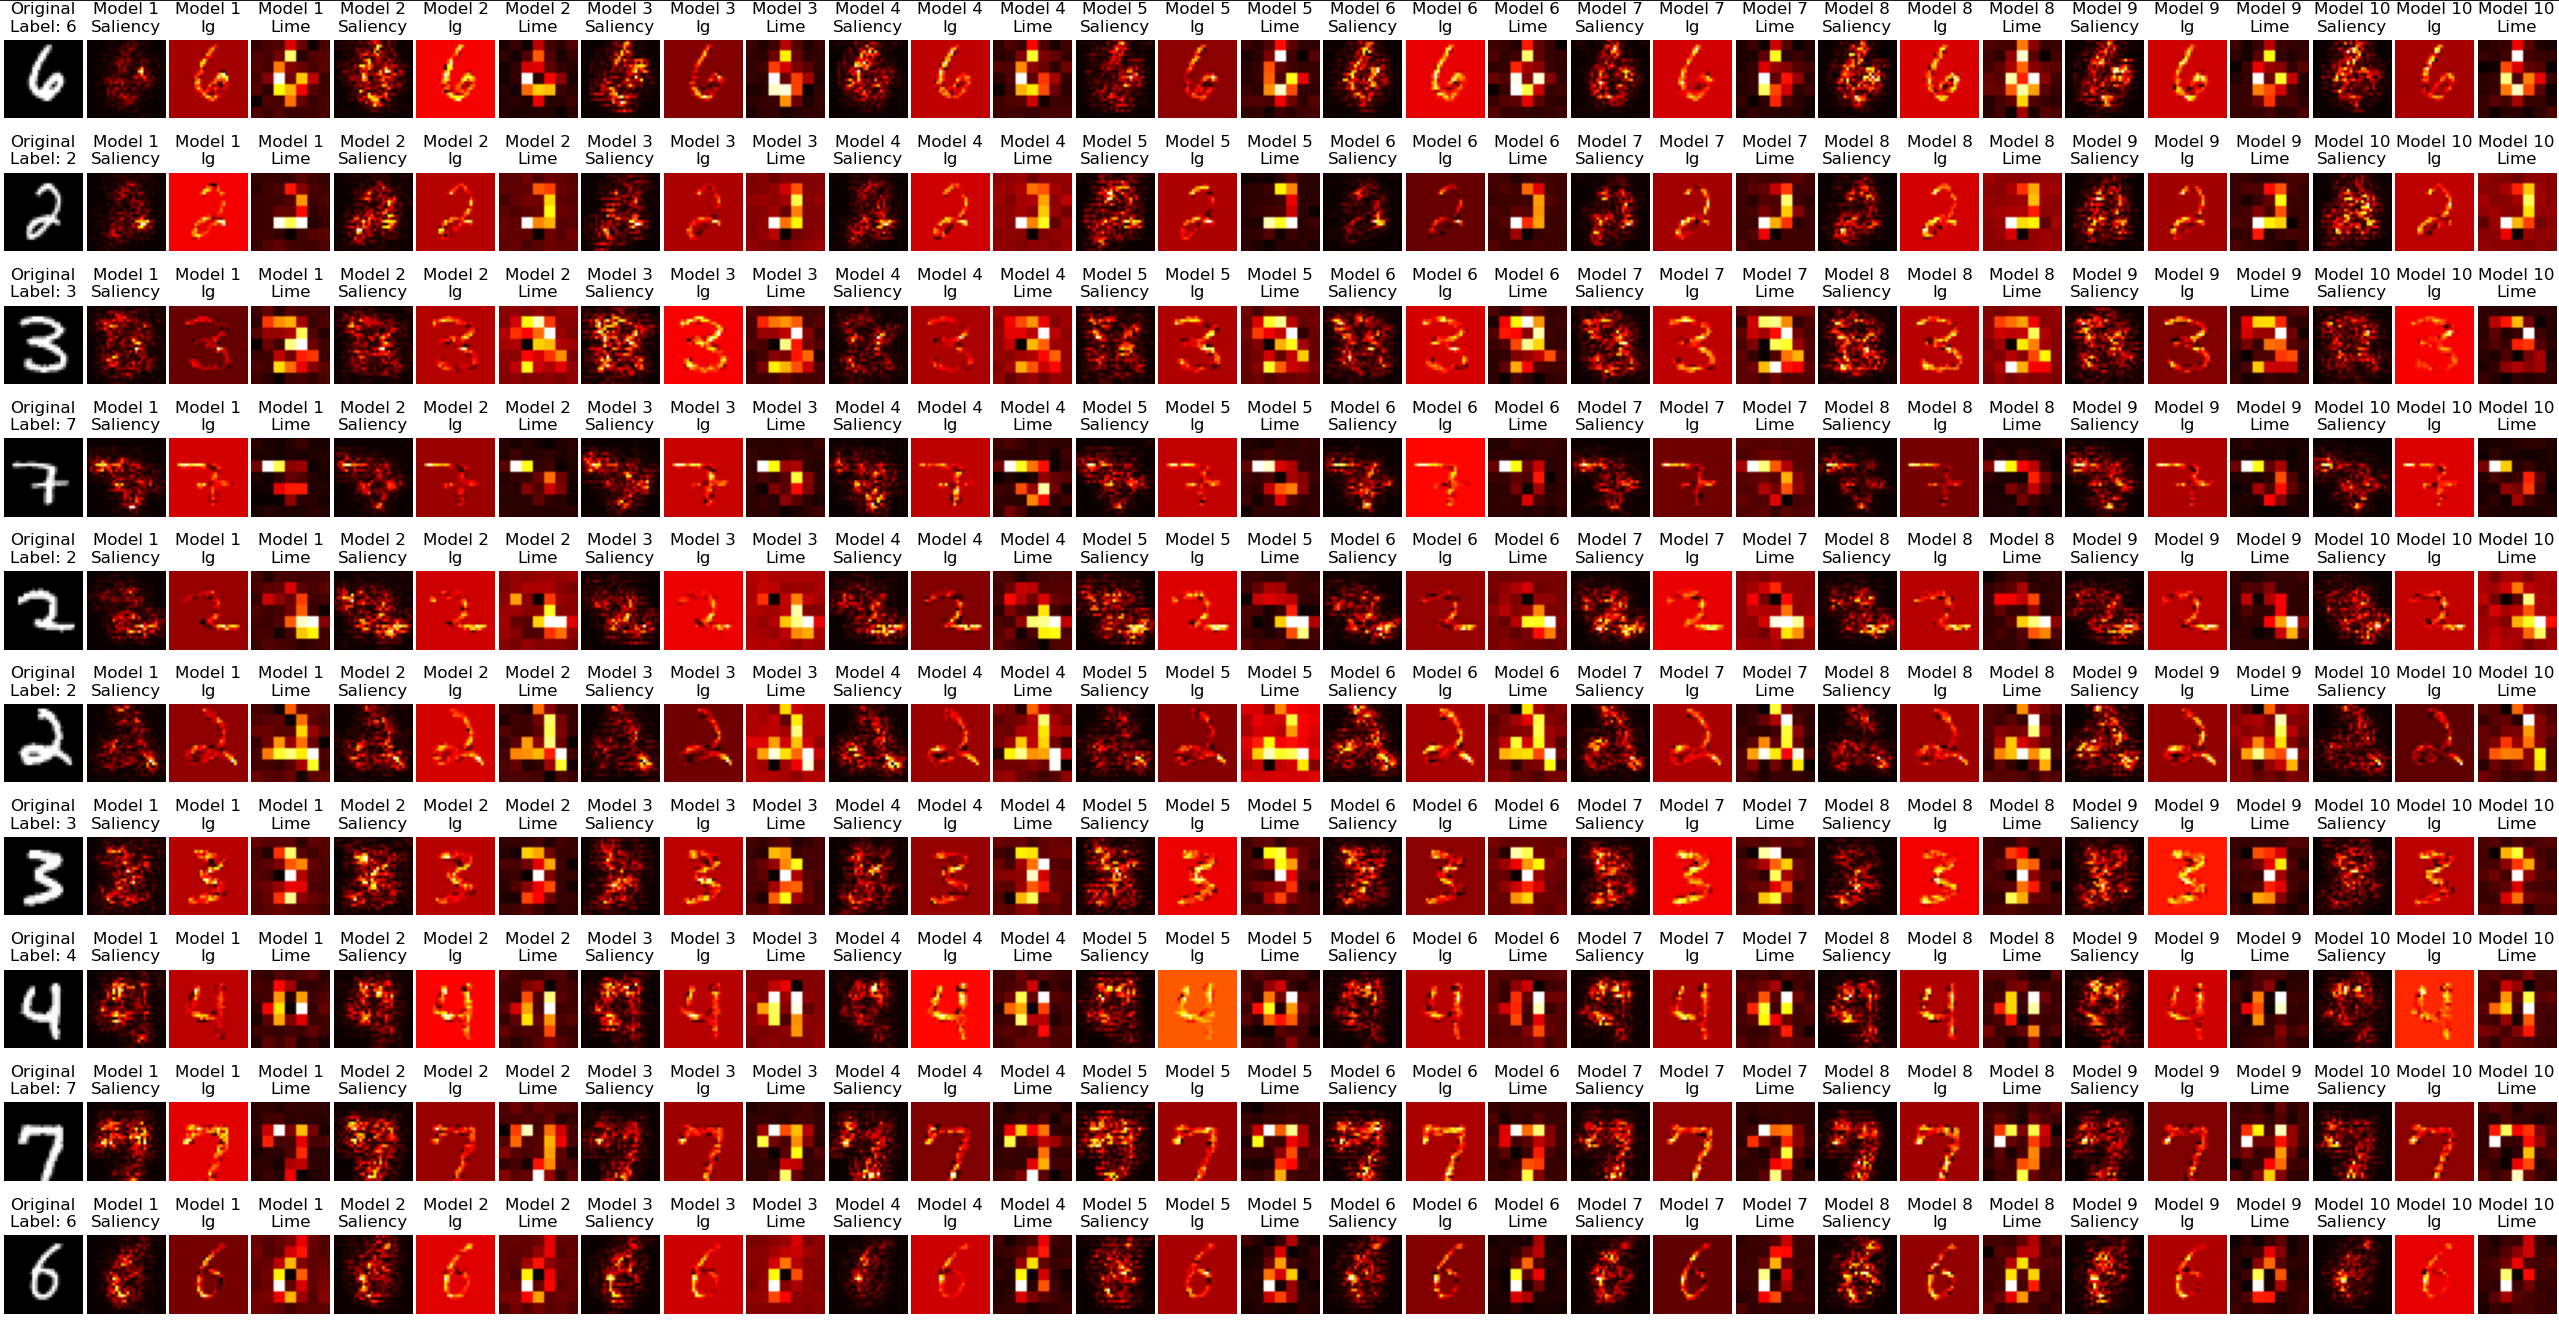
\includegraphics[width=\textwidth]{images/visualizzazione (2).png}
    \caption{Esempi di mappe di attribuzione per 10 modelli del Rashomon set su alcune immagini di test (MNIST). 
    Ogni riga corrisponde a una diversa immagine originale, seguita dalle spiegazioni generate con Saliency, Integrated Gradients (IG) e LIME.
    Si osserva come le spiegazioni siano generalmente più coerenti \textbf{tra modelli} usando lo stesso metodo (colonne verticali), 
    mentre differenze più marcate emergono \textbf{tra metodi} sullo stesso modello (blocchi orizzontali).}
    \label{fig:similarity_examples}
\end{figure}

\subsection{Interpretazione}
I valori mostrano una tendenza chiara:
\begin{itemize}
      \item La similarità \textbf{inter-modello} è molto alta per tutte le metriche,
            segnalando che un singolo metodo tende a produrre spiegazioni coerenti tra
            modelli diversi del Rashomon set.
      \item La similarità \textbf{intra-modello} è significativamente più bassa: metodi
            diversi, anche sullo stesso modello, producono spiegazioni tra loro divergenti.
\end{itemize}

Guardando ai risultati, emerge una tendenza chiara e coerente con quanto
riportato in letteratura: la similarità \textbf{inter-modello} è
sistematicamente più alta della \textbf{intra-modello}, indipendentemente dalla
metrica utilizzata. Questo significa che, una volta scelto un metodo di
spiegazione, le mappe generate rimangono relativamente stabili anche se il
modello cambia — almeno all’interno del Rashomon set considerato. Ad esempio,
LIME raggiunge valori di Pearson sopra $0.90$ tra modelli diversi, mentre la
stessa metrica scende a circa $0.47$–$0.53$ quando si confronta LIME con altri
metodi sullo stesso modello.\\

La situazione si inverte quando cambiamo il metodo: qui le similarità calano
drasticamente, con SSIM intorno a $0.21$–$0.26$ e correlazioni Spearman che, in
certi confronti, non superano $0.22$. Questi numeri confermano che la
\emph{scelta del metodo di spiegazione} è il fattore che più influenza forma,
intensità e posizionamento delle regioni considerate rilevanti. In altre
parole, i metodi “dicono storie diverse” anche quando guardano lo stesso
modello.\\

Questo suggerisce che, nel contesto analizzato, la \emph{scelta del metodo di
      spiegazione} ha un impatto più forte sulla forma e sul contenuto della
spiegazione rispetto alla scelta del modello, almeno all’interno del Rashomon
set considerato.

\section{Valutare la fedeltà delle spiegazioni: MoRF e AOPC}

Misurare la similarità tra spiegazioni è utile per capire se due metodi
``raccontano la stessa storia''. Ma una spiegazione può anche essere coerente e
stabile, eppure irrilevante per il modello. Per questo serve valutare la
\emph{fedeltà}: le feature indicate come rilevanti sono davvero quelle che
guidano la decisione del modello?

\subsection{Procedura MoRF}
Il metodo \emph{Most Relevant First} (MoRF) è un approccio standard in
letteratura per testare la fedeltà delle mappe di importanza. L’idea è
semplice: se le feature indicate come importanti sono davvero decisive,
rimuoverle dovrebbe ridurre rapidamente la confidenza del modello nella classe
target.

Il procedimento seguito è stato il seguente:
\begin{enumerate}
      \item Ordinare le feature o i pixel in base all’importanza decrescente indicata dalla
            mappa.
      \item Mascherare progressivamente le più importanti, in $K=10$ step uguali, partendo
            dalle più rilevanti.
      \item Usare come \emph{baseline} il valore medio dei pixel dell’immagine: questa
            scelta mantiene le immagini \emph{in-distribution}, evitando artefatti dovuti a
            valori estremi come tutto nero o tutto bianco.
      \item Dopo ogni mascheramento, registrare la probabilità che il modello assegna alla
            \textbf{classe vera} (\textit{true label}).
      \item Tracciare la curva MoRF, che mostra il decadimento della confidenza al crescere
            della porzione di immagine mascherata.
\end{enumerate}

\subsection{AOPC: Area Over the Perturbation Curve}
Per riassumere in un solo numero la qualità di una spiegazione, è stata
utilizzata la metrica \textbf{AOPC} (\emph{Area Over the Perturbation Curve}),
calcolata come:

\[
      \mathrm{AOPC} = \frac{1}{K} \sum_{k=1}^K \left[ f(x) - f(x^{(k)}) \right]
\]

dove:
\begin{itemize}
      \item $f(x)$ è la predizione del modello sull’immagine originale.
      \item $f(x^{(k)})$ è la predizione dopo aver mascherato i primi $k$ blocchi di feature più importanti.
      \item $K=10$ è il numero di step di mascheramento.
\end{itemize}

Più il valore AOPC è alto, più la rimozione delle feature considerate
importanti provoca un crollo rapido della confidenza: un segno di elevata
fedeltà della spiegazione.

\subsection{Risultati AOPC}
\begin{table}[h!]
      \centering
      \renewcommand{\arraystretch}{1.1}
      \begin{tabular}{lc}
            \hline
            \textbf{Metodo}      & \textbf{AOPC (media $\pm$ std)} \\
            \hline
            LIME                 & $0.8080 \pm 0.0825$             \\
            Integrated Gradients & $0.7511 \pm 0.1873$             \\
            Saliency             & $0.6568 \pm 0.1495$             \\
            \hline
      \end{tabular}
      \caption{AOPC per metodo (più alto = spiegazione più efficace), $n=100$.}
      \label{tab:aopc_results}
\end{table}

\noindent
I risultati indicano:
\begin{itemize}
      \item \textbf{LIME} provoca il decadimento più rapido della confidenza media, segno che le feature che evidenzia sono spesso effettivamente rilevanti per il modello.
      \item \textbf{Integrated Gradients} ottiene un valore intermedio, combinando buona fedeltà con alta coerenza inter-modello.
      \item \textbf{Saliency} ha valori più bassi, suggerendo che le feature evidenziate non sempre sono decisive per la classificazione.
\end{itemize}

\noindent
Questi valori vanno letti con attenzione. LIME, pur essendo il più rumoroso nelle visualizzazioni e meno coerente tra modelli, ottiene il punteggio AOPC più alto.
Ciò indica che, quando individua una feature come rilevante, questa ha effettivamente un impatto forte sulla decisione del modello.
Integrated Gradients si colloca appena sotto, bilanciando fedeltà elevata e coerenza inter-modello: un compromesso interessante in scenari dove entrambe le proprietà sono desiderabili.
Saliency mostra valori più bassi, suggerendo che alcune feature evidenziate non sono sempre cruciali per la classificazione.

È importante sottolineare che un AOPC alto non implica necessariamente una spiegazione più interpretabile o comprensibile per l’utente umano: misura solo la capacità della spiegazione di identificare feature che, se rimosse, fanno crollare la confidenza del modello.
Inoltre, i valori dipendono da scelte implementative come la baseline di mascheramento (media immagine) e, nel caso di LIME, dalla granularità delle perturbazioni (blocchi $4\times4$) e dal numero di campioni, fattori che influenzano sensibilmente il risultato.

\subsection{Conclusioni}
L’analisi combinata di similarità e fedeltà porta a diverse osservazioni:
\begin{itemize}
      \item La variabilità intra-modello è maggiore di quella inter-modello: il metodo di
            spiegazione influenza più del modello stesso.
      \item LIME eccelle in termini di AOPC, ma soffre di maggiore variabilità e
            rumorosità, specialmente tra modelli diversi.
      \item Integrated Gradients offre un buon compromesso: alta coerenza tra modelli e
            fedeltà elevata.
      \item Saliency è meno performante in entrambi gli aspetti, suggerendo una minore
            utilità pratica nel contesto MNIST.
\end{itemize}

\end{document}
